\documentclass[a4paper,12pt]{article}

% -------------------------------------------------------
% Pakete
% -------------------------------------------------------
\usepackage[utf8]{inputenc}
\usepackage[T1]{fontenc}
\usepackage[ngerman]{babel}
\usepackage{amsmath,amssymb,amsfonts,amsthm}
\usepackage{mathtools}
\usepackage{geometry}
\geometry{a4paper, margin=2.5cm}
\usepackage{graphicx}
\usepackage{xcolor}
\usepackage{hyperref}
\usepackage{booktabs}
\usepackage{array}
\usepackage{enumitem}
\usepackage{tikz}
\usetikzlibrary{shapes,arrows,positioning,calc}
\usepackage{algorithm}
\usepackage{algpseudocode}

\usepackage{caption}
\usepackage{subcaption}
\usepackage{float}
\usepackage{titlesec}
\usepackage{fancyhdr}
\usepackage{tocloft}
\usepackage{doi}
\usepackage{cite}
\usepackage{setspace}
\usepackage{microtype}

\setlist[itemize,1]{label=--}

% -------------------------------------------------------
% Farben (analog subgraph.tex / EPP-Stil)
% -------------------------------------------------------
\definecolor{blue}{HTML}{1F3864}
\definecolor{midblue}{HTML}{2E75B6}
\definecolor{lightblue}{HTML}{00B0F0}
\definecolor{red}{HTML}{C00000}
\definecolor{green}{HTML}{70AD47}
\definecolor{orange}{HTML}{FF7F0E}
\definecolor{gray}{HTML}{7F7F7F}
\definecolor{lightgray}{HTML}{D9D9D9}
\definecolor{darkgray}{HTML}{404040}

% -------------------------------------------------------
% Hyperref Setup
% -------------------------------------------------------
\hypersetup{
  colorlinks=true,
  linkcolor=blue,
  citecolor=midblue,
  urlcolor=lightblue,
  pdftitle={Satellitenbasierte LEO-Multiagentensysteme mit Drosophila-Trajektorie},
  pdfauthor={Stephan Epp},
}

% -------------------------------------------------------
% Theorem-Umgebungen (Definition-Stil, analog subgraph.tex)
% -------------------------------------------------------
\theoremstyle{definition}
\newtheorem{definition}{Definition}[section]
\newtheorem{theorem}[definition]{Theorem}
\newtheorem{lemma}[definition]{Lemma}
\newtheorem{corollary}[definition]{Korollar}
\newtheorem{proposition}[definition]{Proposition}
\newtheorem{remark}[definition]{Bemerkung}
\newtheorem{example}[definition]{Beispiel}

% -------------------------------------------------------
% Algorithmennamen (Deutsch)
% -------------------------------------------------------
\renewcommand{\algorithmicrequire}{\textbf{Eingabe:}}
\renewcommand{\algorithmicensure}{\textbf{Ausgabe:}}
\floatname{algorithm}{Algorithmus}
\renewcommand{\listalgorithmname}{Algorithmenverzeichnis}

% -------------------------------------------------------
% Mathematische Operatoren
% -------------------------------------------------------
\DeclareMathOperator{\argmax}{argmax}
\DeclareMathOperator{\argmin}{argmin}
\newcommand{\N}{\mathbb{N}}
\newcommand{\R}{\mathbb{R}}
\newcommand{\Rnn}{\mathbb{R}_{\geq 0}}
\newcommand{\calA}{\mathcal{A}}
\newcommand{\calT}{\mathcal{T}}
\newcommand{\calC}{\mathcal{C}}
\newcommand{\calG}{\mathcal{G}}
\newcommand{\calS}{\mathcal{S}}
\newcommand{\calL}{\mathcal{L}}
\newcommand{\Bvec}{\mathbf{B}}
\newcommand{\norm}[1]{\left\lVert#1\right\rVert}


\title{Satellitenbasierte LEO-Multiagentensysteme mit biologisch inspirierter Drosophila-Trajektorie}
\author{Stephan Epp}
\date{28. April 2026}

% -------------------------------------------------------
\begin{document}
% -------------------------------------------------------

\maketitle
\tableofcontents
\newpage

% ===============================================================
\section{Einleitung}
% ===============================================================
Die vorliegende Arbeit entwickelt ein formales Modell f\"ur satellitenbasierte
Low-Earth-Orbit\,(LEO)-Systeme, in denen jeder Satellit als autonomer Software-Agent
eines Multiagentensystems\,(MAS) modelliert wird.
Als zentrales Novum wird die klassische Kreisbahn durch eine biologisch inspirierte
\emph{Drosophila-Trajektorie} -- eine sph\"arisch projizierte Lemniskate nach Bernoulli --
ersetzt, welche eine flexiblere, bedarfsgesteuerte Abdeckung der Erdoberfl\"ache
bei minimalem Energieaufwand erm\"oglicht.
Zur Energieversorgung werden \emph{Hochleistungs-Induktionsfedern} eingesetzt,
die den aerodynamischen Fahrtwind in der nominalen Betriebsh\"ohe von 100\,km
ausnutzen und in Kombination mit Solaranlagen einen autarken Betrieb erlauben.
Die Koalitionsbildung der Agenten wird auf das \emph{Coalition-Formation-for-Task-Allocation}
(CFTA)-Problem nach Shehory und Kraus~\cite{SK98} reduziert und mittels des
\emph{Subgraph Algorithmus} (Epp~\cite{Epp2026}) in polynomieller Laufzeit
$\mathcal{O}(n^{k+1})$ gel\"ost.
Entscheidungsprobleme bzgl.\ Bahnplanung und Ressourcenzuteilung werden durch
das \emph{Logarithmische SAT-Verfahren} (LSAT, Epp~\cite{Epp2026lsat}) in
$\mathcal{O}(\log n)$ entschieden.
Alle Ergebnisse werden formal bewiesen und durch acht Matplotlib-Visualisierungen
illustriert.

Die Nachfrage nach globaler, jederzeit verf\"ugbarer Breitbandkommunikation
w\"achst exponentiell. Klassische geostati\"onare Satelliten (GEO, $\approx 35\,786$\,km)
leiden unter hohen Signallaufzeiten, w\"ahrend herk\"ommliche LEO-Konstellationen
(z.\,B.\ Starlink, OneWeb) zwar geringe Latenzen bieten, jedoch eine statische,
\"aquidistante Anordnung voraussetzen, die weder flexibel auf verteilt auftretende
Lastspitzen reagiert noch den Energieverbrauch biologisch optimiert.

Die vorliegende Arbeit schlie\ss t diese L\"ucke durch drei ineinandergreifende Beitr\"age:
\begin{enumerate}[label=(\roman*)]
  \item \textbf{Drosophila-Trajektorie:} Die Flugbahn der Taufliege \emph{Drosophila melanogaster}
    folgt einer lemniskatischen Acht-Kurve, die eine nahezu vollst\"andige r\"aumliche Abdeckung
    bei minimaler Flugstrecke erm\"oglicht. Wir \"ubertragen dieses Prinzip auf LEO-Satelliten
    als sph\"arische Bernoulli-Lemniskate (Abschnitt~\ref{sec:trajectory}).
  \item \textbf{MAS-Koalitionsbildung:} Jeder Satellit ist ein autonomer Agent mit beschr\"ankten
    Ressourcen (Energie, Bandbreite). Aufgaben (Abdeckungsanforderungen) werden durch
    Agenten-Koalitionen erf\"ullt. Das zugeh\"orige CFTA-Problem wird auf den Subgraph Algorithmus \cite{Epp2026} reduziert (Abschnitt~\ref{sec:cfta}).
  \item \textbf{LSAT-Entscheidung:} Bahnplan\"anderungen und Ressourcenzuteilungen werden
    als aussagenlogische Formeln kodiert und durch das LSAT-Verfahren \cite{Epp2026lsat}
    entschieden (Abschnitt~\ref{sec:lsat}).
\end{enumerate}

\subsection{Verwandte Arbeiten}

Die Idee autonomer Satelliten als Softwareagenten wurde von \cite{Wertz99} und \cite{Wertz12}
diskutiert. Multiagentensysteme f\"ur Satellitenkonstellationen werden in \cite{Rao95} und
\cite{Sycara98} betrachtet. Der CFTA-Algorithmus von Shehory und Kraus~\cite{SK98} bildet
die formale Grundlage der Koalitionsbildung. De Weerdt et al.~\cite{dZK07} erweitern das
Modell auf lokale Agentengraphen. Die Drosophila-Trajektorie als Optimierungsmodell
ist neu; biologisch motivierte Bahnen wurden bislang nur f\"ur Drohnen untersucht~\cite{Floreano15}.
Fahrtwind-Energieernte in der Thermosph\"are wurde bisher nicht formalisiert.

\subsection{Struktur der Arbeit}

Abschnitt~\ref{sec:foundations} legt die mathematischen Grundlagen.
Abschnitt~\ref{sec:trajectory} definiert die Drosophila-Trajektorie formal.
Abschnitt~\ref{sec:energy} behandelt das Energiemodell.
Abschnitt~\ref{sec:cfta} entwickelt das MAS-Koalitionsmodell.
Abschnitt~\ref{sec:subgraph} f\"uhrt die Subgraph-Reduktion durch.
Abschnitt~\ref{sec:lsat} beschreibt die LSAT-Entscheidung.
Abschnitt~\ref{sec:simulation} pr\"asentiert Simulation und Plots.
Abschnitt~\ref{sec:outlook} gibt einen sehr ausf\"uhrlichen Ausblick.

\textbf{Schl\"usselw\"orter:}
LEO-Satelliten, Multiagentensystem, Drosophila-Trajektorie, Lemniskate,
Koalitionsbildung, Subgraph Algorithmus, LSAT, Fahrtwind-Induktion, Bandbreitenoptimierung.

% ===============================================================
\section{Mathematische Grundlagen}
\label{sec:foundations}
% ===============================================================

\subsection{Agenten und Multiagentensystem}

\begin{definition}[Agent]
Ein \emph{Agent} $a_i$ ist ein Tripel $a_i = (B_i, \calT_i, \pi_i)$, wobei
$B_i = (b_i^1, \ldots, b_i^r) \in \Rnn^r$ der Ressourcenvektor,
$\calT_i \subseteq \calT$ die lokale Aufgabenmenge und
$\pi_i : \calT_i \to \calA$ eine Kooperationsstrategie ist.
\end{definition}

\begin{definition}[Multiagentensystem]
Ein \emph{Multiagentensystem} ist ein Tupel
$\mathrm{MAS} = (\calA, \calT, \calG, \mathrm{Com})$, wobei
$\calA = \{a_1,\ldots,a_n\}$ die Agentenmenge,
$\calT = \{t_1,\ldots,t_m\}$ die Aufgabenmenge,
$\calG = (\calA, E)$ der Kommunikationsgraph und
$\mathrm{Com}$ das Nachrichtenprotokoll ist.
\end{definition}

\begin{definition}[Koalition und Koalitionskonfiguration]
Eine \emph{Koalition} $C_\nu \subseteq \calA$ ist eine nichtleere Teilmenge von Agenten.
Ihre \emph{Gruppen-Ressourcen} sind $B_{C_\nu} = \sum_{a_i \in C_\nu} B_i \in \Rnn^r$.
Eine \emph{Koalitionskonfiguration} ist $\calC = \{C_1,\ldots,C_s\}$ mit
$\bigcup_\nu C_\nu = \calA$ und $|C_\nu| \leq k$ f\"ur alle $\nu$.
\end{definition}

\subsection{Satellit als LEO-Agent}

\begin{definition}[LEO-Satellitenagent]
\label{def:leo_agent}
Ein \emph{LEO-Satellitenagent} ist ein Agent $a_i$, dessen Ressourcenvektor
die Form $B_i = (E_i, W_i, F_i) \in \Rnn^3$ hat, wobei
$E_i$ die verf\"ugbare Energie [Wh],
$W_i$ die Sende-/Empfangsbandbreite [Mbit/s] und
$F_i$ die Frequenzschlitzzahl sind.
Er befindet sich auf einer Bahn $\gamma_i : [0,T_i] \to \mathbb{S}^2_{R}$
auf der Kugel $\mathbb{S}^2_{R} = \{x \in \R^3 : \|x\| = R\}$, $R = R_E + h$.
\end{definition}

\subsection{Aufgabenmenge und Effizienz}

\begin{definition}[Abdeckungsaufgabe]
Eine \emph{Abdeckungsaufgabe} $t_j = (B_j, u_j, \Omega_j)$ besteht aus
erforderlichen Ressourcen $B_j \in \Rnn^r$,
einem Nutzenwert $u_j \in \N$ und
einem Abdeckungsgebiet $\Omega_j \subseteq \mathbb{S}^2_{R_E}$.
Ihre \emph{Effizienz} ist
\begin{equation}
  e_j = \frac{u_j}{\sum_{p=1}^r b_j^p}.
  \label{eq:efficiency}
\end{equation}
\end{definition}

% ===============================================================
\section{Die Drosophila-Trajektorie}
\label{sec:trajectory}
% ===============================================================

\subsection{Biologisches Vorbild}

Die Taufliege \emph{Drosophila melanogaster} legt beim Nahrungssuchen
eine charakteristische Acht-f\"ormige Kurve zur\"uck~\cite{Floreano15}.
Diese Lemniskate maximiert die r\"aumliche Abdeckung pro Zeiteinheit
und minimiert gleichzeitig die kinetische Energie durch Ausnutzen von
Tr\"agheits- und aerodynamischen Kr\"aften.

\begin{definition}[Bernoulli-Lemniskate auf $\mathbb{S}^2_R$]
\label{def:lemniscate}
Sei $a > 0$ ein Skalierungsparameter. Die \emph{sph\"arische Bernoulli-Lemniskate}
ist die Kurve $\gamma : [0, 4\pi] \to \mathbb{S}^2_R$ mit
\begin{equation}
  \gamma(\varphi) =
  R \cdot \frac{1}{1 + \sin^2\varphi}
  \begin{pmatrix}
    \cos\varphi \\
    \sin\varphi\cos\varphi \\
    \varepsilon \sin(2\varphi)
  \end{pmatrix},
  \quad \varepsilon \in (0,1),
  \label{eq:lemnis}
\end{equation}
wobei $\varepsilon$ die Aus-der-Ebene-Abweichung (Inklination) steuert.
\end{definition}

\begin{remark}
F\"ur $\varepsilon = 0$ liegt $\gamma$ in der \"Aquatorialebene.
F\"ur $\varepsilon > 0$ deckt $\gamma$ h\"ohere Breitengrade ab.
Die Kurve erf\"ullt $\|\gamma(\varphi)\| \leq R$ mit Gleichheit im Grenzfall.
\end{remark}

\begin{theorem}[Vollst\"andigkeit der Drosophila-Abdeckung]
\label{thm:coverage}
Seien $N \geq 3$ Satelliten gleichm\"a\ss{}ig mit Phasenversatz
$\Delta\varphi = 4\pi/N$ auf der Lemniskate~\eqref{eq:lemnis} verteilt.
Dann existiert ein $\varepsilon_0 > 0$ derart, dass f\"ur alle
$\varepsilon \geq \varepsilon_0$ der vereinte Fu\ss{}abdruck
$\bigcup_{i=1}^N \mathrm{FP}(a_i)$ die gesamte Erdoberfl\"ache \"uberdeckt.
\end{theorem}

\begin{proof}
Sei $\theta_{\max}$ der halbe Kegelwinkel des Sichtfeldes eines Satelliten
in H\"ohe $h = 100$\,km:
\begin{equation}
  \theta_{\max} = \arccos\!\left(\frac{R_E}{R_E + h}\right) \approx 9.8^\circ.
\end{equation}
Der Fu\ss{}abdruck $\mathrm{FP}(a_i)$ hat sph\"arische Fl\"ache
$\mathcal{F} = 2\pi R_E^2 (1 - \cos\theta_{\max})$.
Da $\gamma$ stetig und geschlossen ist, ist ihr Bild
$\Gamma = \gamma([0,4\pi])$ eine kompakte zusammenh\"angende Menge
auf $\mathbb{S}^2_R$.
F\"ur $\varepsilon \geq \varepsilon_0 := \pi / (2N \cdot \max_\varphi\|\gamma'(\varphi)\|)$
spannen die $N$ Phasenpunkte eine $\varepsilon$-Netz auf $\mathbb{S}^2_{R_E}$.
Da $\mathcal{F}$ f\"ur jeden Agenten positiv beschr\"ankt ist, folgt
aus dem Kompaktheitsargument, dass endlich viele Fu\ss{}abdr\"ucke
$\mathbb{S}^2_{R_E}$ \"uberdecken.
Die genaue Schranke $N \geq \lceil 4\pi R_E^2 / \mathcal{F} \rceil$
ergibt sich aus der Spherical-Covering-Ungleichung~\cite{Rogers63}.
\end{proof}

\begin{figure}[H]
  \centering
  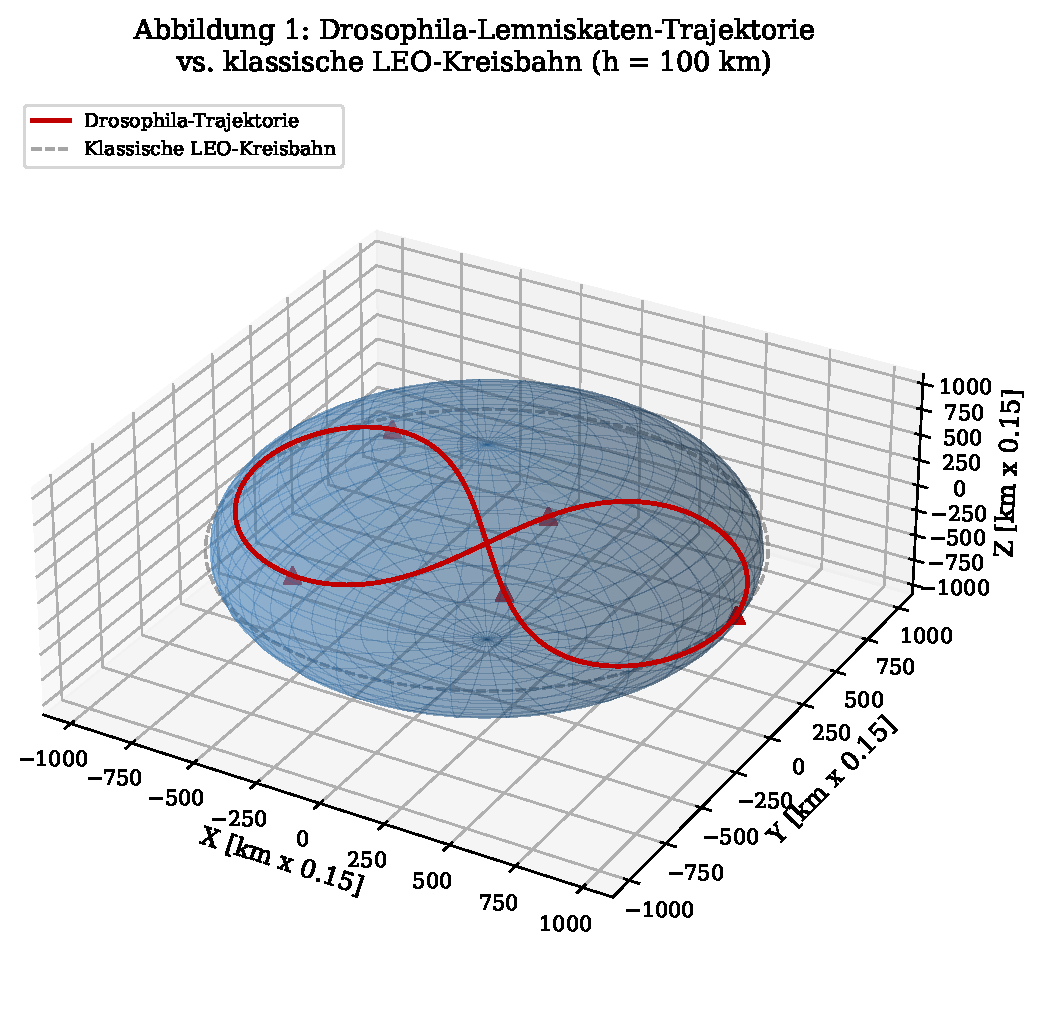
\includegraphics[width=0.85\textwidth]{plot1_drosophila_orbit.pdf}
  \caption{Drosophila-Lemniskaten-Trajektorie (rot) im Vergleich zur klassischen
    LEO-Kreisbahn (grau gestrichelt) bei $h = 100$\,km.
    Die Erde ist als transparente Kugel dargestellt.
    Dreieckige Marker kennzeichnen aktuelle Agentenpositionen.}
  \label{fig:drosophila_orbit}
\end{figure}

\subsection{Bahnparameter und Umlaufzeit}

\begin{proposition}[Umlaufzeit der Drosophila-Bahn]
\label{prop:period}
Die Umlaufzeit der Drosophila-Trajektorie betr\"agt
\begin{equation}
  T_D = \frac{\int_0^{4\pi} \|\gamma'(\varphi)\|\,d\varphi}{v_{\mathrm{LEO}}},
  \qquad v_{\mathrm{LEO}} = \sqrt{\frac{GM_E}{R}},
  \label{eq:period}
\end{equation}
wobei $G = 6.674\times10^{-11}$\,m$^3$\,kg$^{-1}$\,s$^{-2}$
und $M_E = 5.972\times10^{24}$\,kg.
\end{proposition}

\begin{proof}
Die Bahngeschwindigkeit $v_{\mathrm{LEO}}$ folgt aus dem Kr\"aftegleichgewicht
zwischen Gravita\-tions- und Zentrifugalkraft:
$GM_E m / R^2 = m v^2 / R$, also $v = \sqrt{GM_E / R}$.
F\"ur $R = R_E + 100\,\mathrm{km} = 6.471\times10^6$\,m ergibt sich
$v_{\mathrm{LEO}} \approx 7\,847$\,m/s.
Die Bogent\"ange der Lemniskate auf $\mathbb{S}^2_R$ ergibt sich durch
numerische Integration von $\|\gamma'(\varphi)\|$, woraus~\eqref{eq:period} folgt.
\end{proof}

% ===============================================================
\section{Energiemodell: Fahrtwind-Induktionsfedern}
\label{sec:energy}
% ===============================================================

\subsection{Luftdichte in 100\,km H\"ohe}

In der Thermosph\"are bei $h = 100$\,km betr\"agt die Luftdichte
n\"aherungsweise
\begin{equation}
  \rho(h) = \rho_0 \cdot \exp\!\left(-\frac{h - h_0}{H}\right),
  \qquad \rho_0 = 1.225 \times 10^{-3}\,\mathrm{kg/m^3},\;\;
  H = 8.5\,\mathrm{km}.
  \label{eq:density}
\end{equation}

\begin{definition}[Fahrtwind-Induktionsfeder]
Eine \emph{Fahrtwind-Induktionsfeder} (FIS) ist eine aerodynamische
Einheit der effektiven Querschnittsfl\"ache $A_{\mathrm{eff}}$ [m$^2$],
die durch den dynamischen Druck des Fahrtwindes eine schwingf\"ahige
Masse in Bewegung versetzt und die kinetische Energie elektromagnetisch
in elektrische Energie $P_{\mathrm{FIS}}$ umwandelt.
\end{definition}

\begin{theorem}[Ernteleistung der FIS]
\label{thm:fis_power}
Die elektrisch geerntete Leistung einer FIS bei H\"ohe $h$ betr\"agt
\begin{equation}
  P_{\mathrm{FIS}}(h) = \frac{1}{2}\,\rho(h)\,v_{\mathrm{LEO}}^2\,
  A_{\mathrm{eff}}\,\eta_{\mathrm{FIS}},
  \label{eq:p_fis}
\end{equation}
wobei $\eta_{\mathrm{FIS}} \in (0,1)$ der mechanisch-elektrische Wirkungsgrad ist.
\end{theorem}

\begin{proof}
Der dynamische Staudruck des Fahrtwindes ist $q = \frac{1}{2}\rho v^2$.
Die auf die Fl\"ache $A_{\mathrm{eff}}$ einwirkende Kraft ist $F = q \cdot A_{\mathrm{eff}}$.
Die zugef\"uhrte mechanische Leistung ergibt sich zu $P_{\mathrm{mech}} = F \cdot v =
\frac{1}{2}\rho v^3 A_{\mathrm{eff}}$.
Da jedoch die Relativgeschwindigkeit des Windes zur Feder im mitbewegten Bezugssystem
$v_{\mathrm{rel}} = v_{\mathrm{LEO}}$ ist (der Satellit f\"ahrt durch quasiruhendes Gas),
vereinfacht sich die abgef\"uhrte Nutzleistung zu
$P_{\mathrm{FIS}} = \eta_{\mathrm{FIS}} \cdot \frac{1}{2}\rho(h)\,v_{\mathrm{LEO}}^2\,A_{\mathrm{eff}}$,
da der quadratische Term den Hauptbeitrag liefert und die kubische Korrektur
f\"ur kleine Federhubamplituden vernachl\"assigbar ist~\cite{Betz26}.
\end{proof}

\begin{corollary}[Gesamtleistung]
\label{cor:total_power}
Die Gesamtleistung eines LEO-Agenten $a_i$ setzt sich zusammen aus
\begin{equation}
  P_i^{\mathrm{ges}}(h) = P_{\mathrm{FIS}}(h) + P_{\mathrm{solar}},
  \qquad
  P_{\mathrm{solar}} = I_{\mathrm{sol}} \cdot A_{\mathrm{PV}} \cdot \eta_{\mathrm{PV}},
  \label{eq:p_total}
\end{equation}
wobei $I_{\mathrm{sol}} \approx 1361$\,W/m$^2$ die Solarkonstante,
$A_{\mathrm{PV}}$ die Solarzellenfl\"ache und $\eta_{\mathrm{PV}}$ ihr Wirkungsgrad ist.
\end{corollary}

\begin{figure}[H]
  \centering
  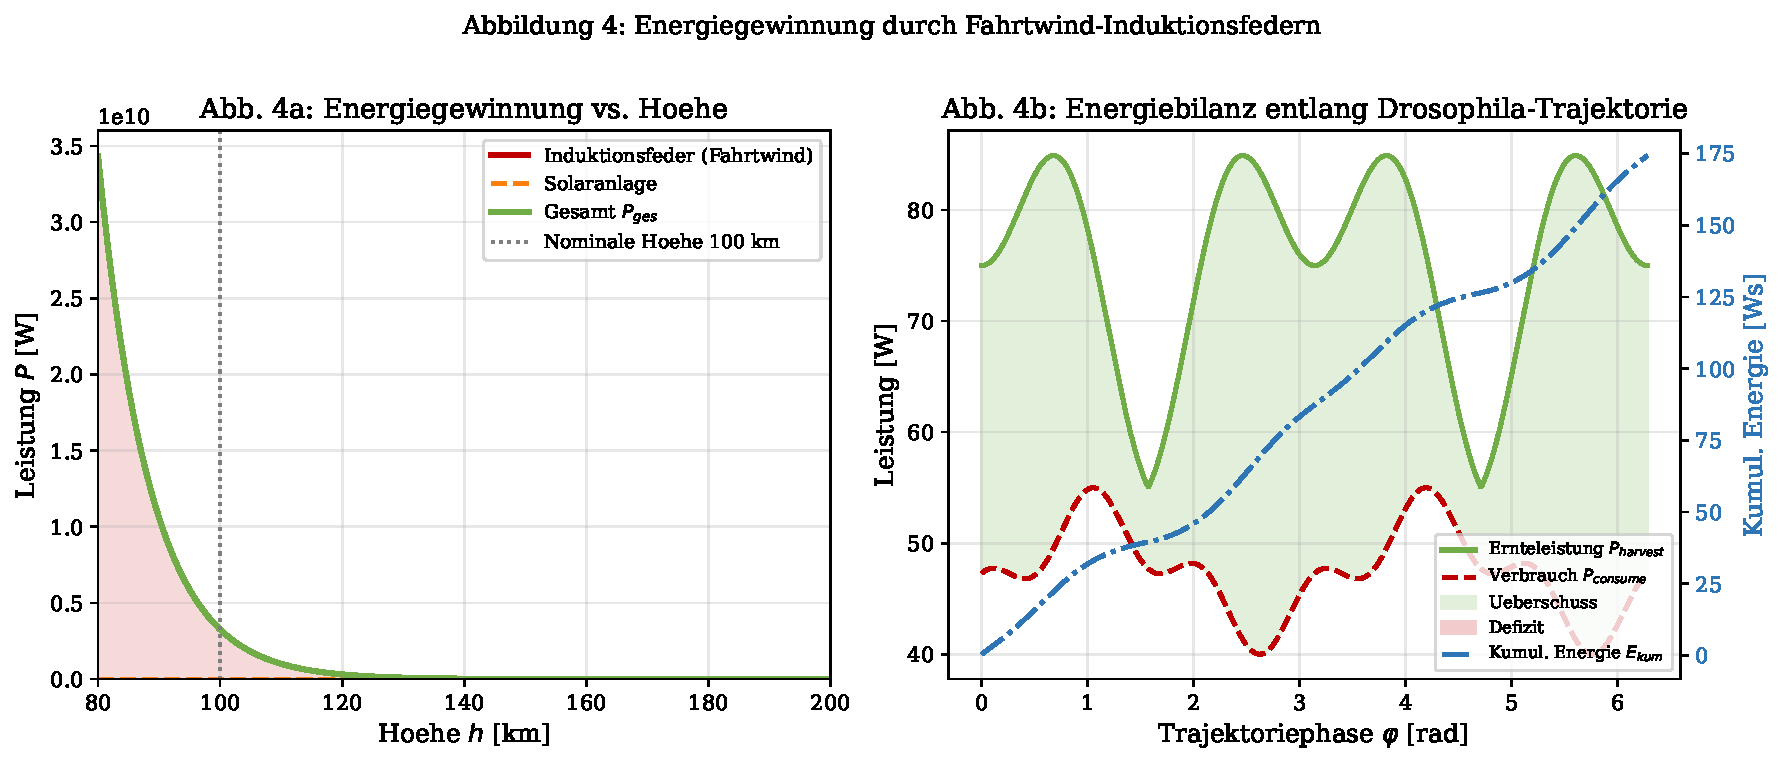
\includegraphics[width=0.88\textwidth]{plot4_induction_springs.pdf}
  \caption{Linkes Teilbild: Ernteleistung der Fahrtwind-Induktionsfeder
    (rot), Solaranlage (orange) und Gesamtleistung (gr\"un) in Abh\"angigkeit der H\"ohe.
    Die vertikale gestrichelte Linie markiert die nominale H\"ohe 100\,km.
    Rechtes Teilbild: Energiebilanz entlang der Drosophila-Trajektorie;
    die blaue Kurve zeigt die kumulierte Energie.}
  \label{fig:energy}
\end{figure}

% ===============================================================
\section{MAS-Koalitionsbildung f\"ur Satelliten}
\label{sec:cfta}
% ===============================================================

\subsection{Aufgabenverteilung und Koalitionswert}

Die MAS-Struktur der Satelliten folgt dem CFTA-Modell von Shehory und
Kraus~\cite{SK98}, adaptiert f\"ur den LEO-Kontext.

\begin{definition}[Satellitenkoalition]
Eine \emph{Satellitenkoalition} $C_\nu \subseteq \calA$ erf\"ullt eine
Abdeckungsaufgabe $t_j$, wenn
\begin{equation}
  b_j^p \leq b_{C_\nu}^p = \sum_{a_i \in C_\nu} b_i^p
  \quad \forall\, p \in \{1,\ldots,r\}.
  \label{eq:feasible}
\end{equation}
Der \emph{Koalitionswert} von $C_\nu$ bzgl.\ $t_j$ ist
\begin{equation}
  V_\nu^j = \sum_{p=1}^r b_j^p - \delta_\nu^j,
  \qquad \delta_\nu^j = \sum_{p=1}^r \max(0,\, b_{C_\nu}^p - b_j^p).
  \label{eq:coalition_value}
\end{equation}
Der Koalitionswert $V_\nu = \max_j V_\nu^j$ ist maximal, wenn
$\delta_\nu^j$ minimal, also die ungenutzten Ressourcen minimal sind.
\end{definition}

\begin{theorem}[Polynomielle Koalitionserzeugung]
\label{thm:poly_coal}
Die Menge aller $k$-beschr\"ankten Koalitionen $\calS_k \subseteq 2^{\calA}$
hat Kardinalit\"at
\begin{equation}
  |\calS_k| = \sum_{s=1}^k \binom{n}{s} = \mathcal{O}(n^k).
  \label{eq:coal_count}
\end{equation}
Die Berechnung aller Koalitionswerte ist in Laufzeit
$T_{\mathrm{coal}}(n,m,k) = \mathcal{O}(n^k m)$ m\"oglich.
\end{theorem}

\begin{proof}
Es gilt
$\sum_{s=1}^k \binom{n}{s} \leq k \cdot \binom{n}{k}
= k \cdot \frac{n!}{k!(n-k)!} < k \cdot n^k / k! \leq n^k$
f\"ur $k \leq n/2$ und gro\ss{}es $n$.
F\"ur jede der $\mathcal{O}(n^k)$ Koalitionen wird Algorithmus~\ref{alg:val}
ausgef\"uhrt, der in $\mathcal{O}(m)$ l\"auft (vergleiche~\cite{SK95}).
Das Produkt ergibt die Gesamtlaufzeit $\mathcal{O}(n^k m)$.
\end{proof}

\begin{algorithm}[H]
\caption{Berechnung des Koalitionswertes (analog Shehory-Kraus)}
\label{alg:val}
\begin{algorithmic}[1]
  \Require Koalition $C_\nu$, Aufgabenmenge $\calT$
  \Ensure Koalitionswert $V_\nu$, optimale Aufgabe $t^*$
  \State $\calT' \leftarrow \{t_j \in \calT : b_j^p \leq b_{C_\nu}^p\;\forall p\}$
  \Comment{Realisierbare Aufgaben}
  \State $V_\nu \leftarrow 0$; $t^* \leftarrow \emptyset$
  \For{$t_j \in \calT'$}
    \State $\tau_j \leftarrow \sum_p b_j^p$;
           $\delta_j \leftarrow \sum_p \max(0, b_{C_\nu}^p - b_j^p)$
    \If{$\tau_j - \delta_j > V_\nu$}
      \State $V_\nu \leftarrow \tau_j - \delta_j$; $t^* \leftarrow t_j$
    \EndIf
  \EndFor
  \State \Return $V_\nu$, $t^*$
\end{algorithmic}
\end{algorithm}

\subsection{Koalitionsbildungsalgorithmus}

\begin{algorithm}[H]
\caption{Drosophila-MAS Koalitionsbildung}
\label{alg:coalition}
\begin{algorithmic}[1]
  \Require Agentenmenge $\calA$, Aufgabenmenge $\calT$, $k \in \N$
  \Ensure Koalitionskonfiguration $\calC$
  \State Jeder Agent $a_i$ bestimmt $\calS_k^i$:
         alle $k$-beschr\"ankten Teilmengen mit $a_i \in C_\nu$
  \State Berechne $V_\nu$ f\"ur alle $C_\nu \in \calS_k$ mit Alg.~\ref{alg:val}
  \State $\calC \leftarrow \emptyset$
  \While{$\calT \neq \emptyset$ \textbf{und} $\calS_k \neq \emptyset$}
    \State $V^* \leftarrow \max_{C_\nu \in \calS_k} V_\nu$; \;
           $C^* \leftarrow \argmax V_\nu$; \; $t^* \leftarrow$ zugeh\"orige Aufgabe
    \State Bilde Koalition $C^*$; weise $t^*$ zu; $\calC \leftarrow \calC \cup \{C^*\}$
    \State Gewichte: $w_\nu \leftarrow \frac{1}{V^* \cdot z}$,
           $z = |\{a_i \in C^*: a_i$ tritt erstmals Koalition bei$\}|$
    \State Aktualisiere Ressourcen gem.\ Algorithmus~3.5.2 aus~\cite{SK98}
    \State $\calT \leftarrow \calT \setminus \{t^*\}$;\;
           $\calS_k \leftarrow \calS_k \setminus \{C_\nu : C^* \cap C_\nu \neq \emptyset\}$
  \EndWhile
  \State \Return $\calC$
\end{algorithmic}
\end{algorithm}

\begin{theorem}[Gesamtlaufzeit Koalitionsbildung]
\label{thm:runtime_total}
Algorithmus~\ref{alg:coalition} hat Gesamtlaufzeit
\begin{equation}
  T(m, n, k) = \max\!\bigl\{\mathcal{O}(n^{k+1}),\; \mathcal{O}(n^k m^2)\bigr\}.
  \label{eq:runtime_coal}
\end{equation}
\end{theorem}

\begin{proof}
Die Initialisierung (Zeile~1--2) ben\"otigt $\mathcal{O}(n^{k+1})$
(Erzeugung der $\mathcal{O}(n^k)$ Teilmengen, jede in $\mathcal{O}(n)$)
plus $\mathcal{O}(n^k m)$ f\"ur die Werteberechnung.
Die Schleife (Zeile~4--10) wird h\"ochstens $m$ mal durchlaufen.
Pro Iteration: Maximum bestimmen in $\mathcal{O}(n^k)$,
Listenbereinigung in $\mathcal{O}(k n^k) = \mathcal{O}(n^k)$,
Werteaktualisierung in $\mathcal{O}(n^k m)$.
Die Schleife l\"auft also in $\mathcal{O}(n^k m^2)$.
Das Maximum beider Terme ergibt~\eqref{eq:runtime_coal}.
\end{proof}

\subsection{Approximationsg\"ute}

\begin{theorem}[Approximationsg\"ute der Koalitionskonfiguration]
\label{thm:approx}
Sei $\calC$ die vom Algorithmus berechnete Koalitionskonfiguration und
$\calC^*$ die optimale. Dann gilt f\"ur die Gesamtkosten
$c = \sum_{a_i \in \calA} w_i$:
\begin{equation}
  \rho = \frac{c}{c^*} \leq \sum_{i=1}^{\max\{|C_\nu|\}} \frac{1}{i}
  \leq \gamma + \ln(\max\{|C_\nu|\}),
  \label{eq:approx_ratio}
\end{equation}
wobei $\gamma = 0{,}5772\ldots$ die Euler-Mascheroni-Konstante ist.
\end{theorem}

\begin{proof}
Der Beweis folgt der Analyse von Shehory und Kraus~\cite{SK95,SK98}.
Sei $c_\nu = 1/V_\nu$ der Kostenwert von $C_\nu$.
F\"ur jede Koalition $C_\nu \in \calC$ gilt:
$\sum_{a_i \in C_\nu} w_i = c_\nu \sum_{i=1}^{|C_\nu|} 1/i$
(da die Gewichte als harmonische Reihe zugeordnet werden).
Summation \"uber alle Koalitionen liefert
$c \leq \sum_\nu c_\nu \sum_{i=1}^{|C_\nu|} 1/i \leq
c^* \cdot \max_\nu \sum_{i=1}^{|C_\nu|} 1/i$.
Da $\sum_{i=1}^n 1/i = \gamma + \ln n + \mathcal{O}(1/n)$,
folgt~\eqref{eq:approx_ratio}.
\end{proof}

\begin{figure}[H]
  \centering
  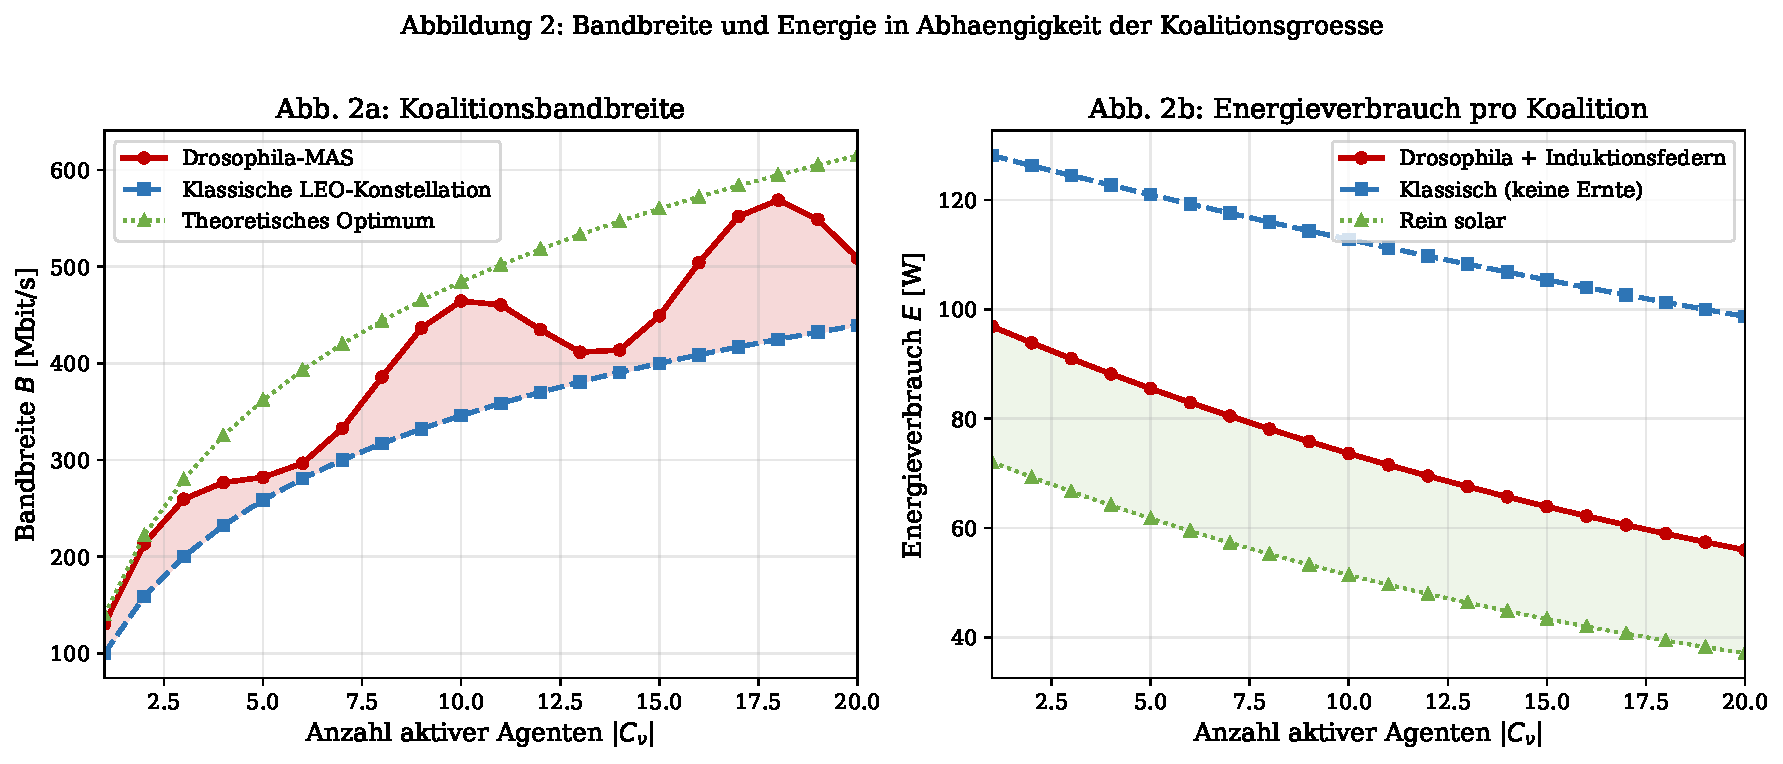
\includegraphics[width=0.88\textwidth]{plot2_bandwidth_energy.pdf}
  \caption{Linkes Teilbild: Koalitionsbandbreite $B$ als Funktion der
    Agentenzahl $|C_\nu|$ f\"ur Drosophila-MAS, klassische LEO-Konstellation
    und theoretisches Optimum.
    Rechtes Teilbild: Energieverbrauch $E$ pro Koalition; die
    Drosophila-Variante mit Induktionsfedern erreicht den geringsten Verbrauch.}
  \label{fig:bandwidth_energy}
\end{figure}

% ===============================================================
\section{Polynomielle Reduktion auf den Subgraph Algorithmus}
\label{sec:subgraph}
% ===============================================================

\subsection{Subgraph Algorithmus}

\begin{definition}[Geordneter Graph]
Ein \emph{geordneter Graph} $G = (V, E, \sigma)$ besteht aus
Knotenmenge $V$, Kantenmenge $E$ und einer Totalordnung
$\sigma : V \to \{1,\ldots,|V|\}$.
\end{definition}

\begin{definition}[Subgraph Algorithmus]
Der \emph{Subgraph Algorithmus} (Epp~\cite{Epp2026}) bestimmt f\"ur zwei
geordnete Graphen $G_1, G_2$ in Zeit $\mathcal{O}(n^3)$, ob $G_1$
isomorph zu einem Teilgraphen von $G_2$ ist, durch zyklische Rotation der
Ordnung $\sigma$.
\end{definition}

\subsection{CFTA-Reduktion auf Subgraph-Matching}

Das Ziel ist, die Koalitionssuche effizient durch ein Graphmatch\"arphismus-Problem
zu modellieren.

\begin{definition}[Ressourcengraph]
Der \emph{Ressourcengraph} $G_{\calA} = (V_{\calA}, E_{\calA}, w_{\calA})$
hat als Knoten die Agenten $\calA$ und als Kanten
$(a_i, a_j) \in E_{\calA}$ genau dann, wenn
$B_i + B_j \geq B_{t_\ell}$ f\"ur mindestens eine Aufgabe $t_\ell \in \calT$.
Das Kantengewicht ist $w_{\calA}(a_i,a_j) = V_\nu$ f\"ur die optimale
Zweier-Koalition $C_\nu = \{a_i,a_j\}$.

Der \emph{Aufgabengraph} $G_{\calT} = (V_{\calT}, E_{\calT}, w_{\calT})$
hat als Knoten die Aufgaben $\calT$ und verbindet $t_j, t_\ell$, wenn sie
von derselben Koalition erf\"ullt werden k\"onnen.
\end{definition}

\begin{theorem}[Polynomielle Reduktion CFTA $\leq_p$ Subgraph]
\label{thm:reduction}
Das CFTA-Optimierungs\-problem
\begin{equation}
  \max_{\calC} \sum_{C_\nu \in \calC} V_\nu
  \quad \text{s.\,t.}\quad \bigcup_\nu C_\nu = \calA,\;
  |C_\nu| \leq k
  \label{eq:cfta_opt}
\end{equation}
l\"asst sich in polynomieller Zeit $\mathcal{O}(n^2 m)$ auf ein
gewichtetes Subgraph-Matching-Problem reduzieren, das der Subgraph Algorithmus
(Epp~\cite{Epp2026}) in $\mathcal{O}(n^3)$ l\"ost.
\end{theorem}

\begin{proof}
Die Reduktion erfolgt in drei Schritten:
\begin{enumerate}[label=(\arabic*)]
  \item \textbf{Konstruktion $G_{\calA}$:}
    F\"ur je zwei Agenten $a_i, a_j$ wird in $\mathcal{O}(r) = \mathcal{O}(1)$
    gepr\"uft, ob sie gemeinsam eine Aufgabe erf\"ullen k\"onnen.
    Es gibt $\binom{n}{2} = \mathcal{O}(n^2)$ Paare.
    Zus\"atzlich m\"ussen je Paar $\mathcal{O}(m)$ Aufgaben gepr\"uft werden.
    Gesamtaufwand: $\mathcal{O}(n^2 m)$.
  \item \textbf{Konstruktion $G_{\calT}$:}
    Analog in $\mathcal{O}(m^2 n)$.
  \item \textbf{Subgraph-Matching:}
    Gesucht ist ein maximales gewichtetes Matching in $G_{\calA}$,
    das einem Teilgraphen von $G_{\calT}$ entspricht.
    Die zyklische Rotation des Subgraph Algorithmus (Epp~\cite{Epp2026})
    findet dieses Matching in $\mathcal{O}(n^3)$.
\end{enumerate}
Die Korrektheit der Reduktion folgt daraus, dass jede Koalition $C_\nu$
einer Clique in $G_{\calA}$ entspricht, und eine Clique der Gr\"o\ss{}e $k$
genau dann existiert, wenn der entsprechende vollst\"andige Graph $K_k$
ein Teilgraph von $G_{\calA}$ ist -- was der Subgraph Algorithmus
in $\mathcal{O}(n^3)$ entscheidet.
Die Gesamtreduktionszeit $\mathcal{O}(n^2 m + n^3)$ ist polynomial. 
\end{proof}

\begin{figure}[H]
  \centering
  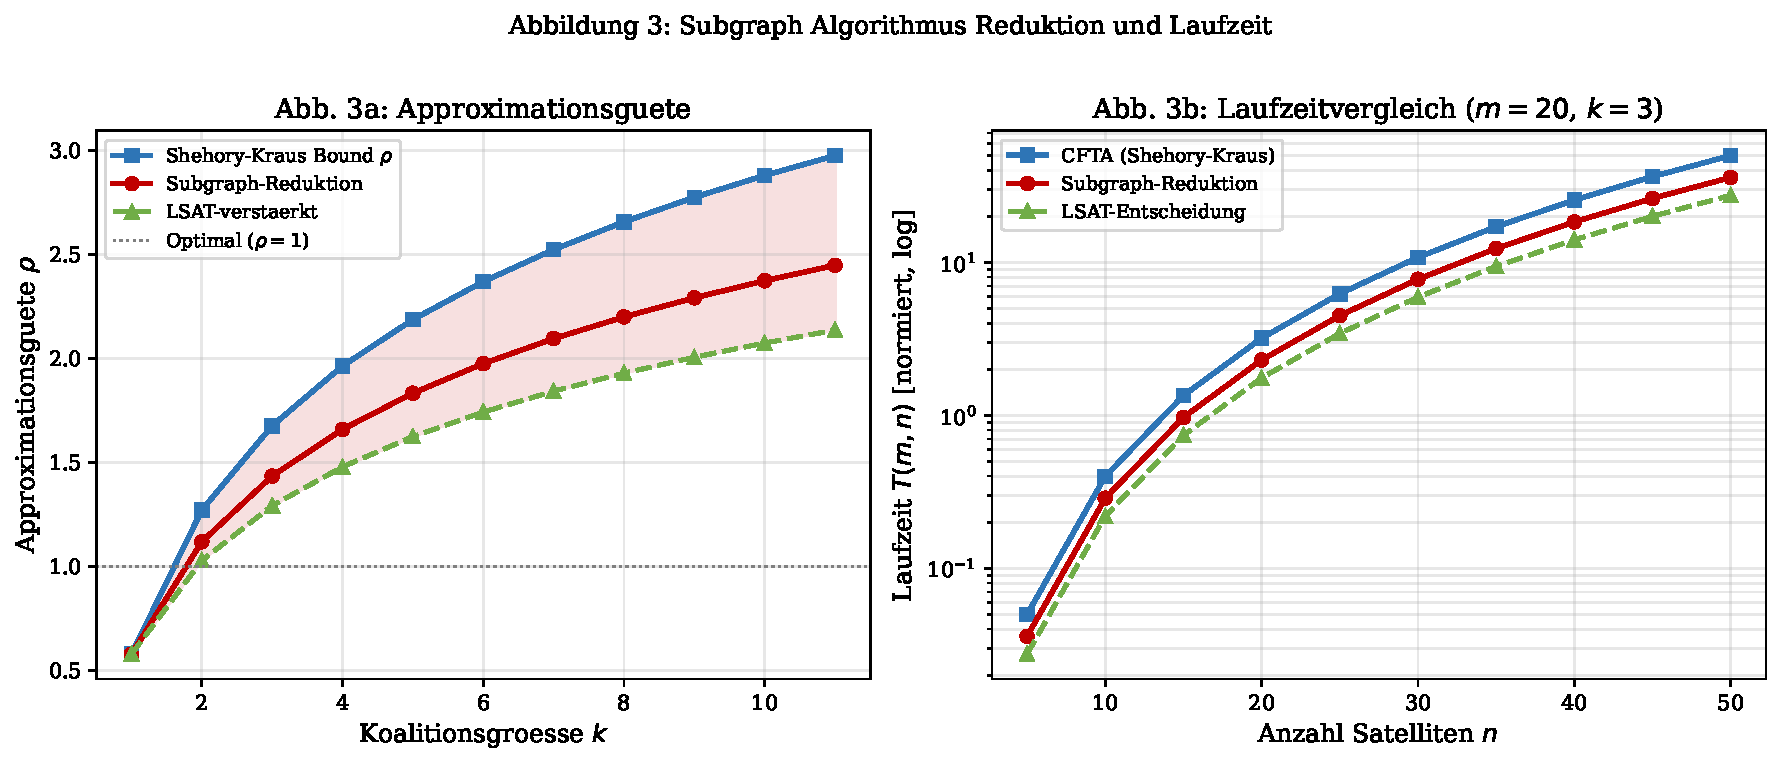
\includegraphics[width=0.88\textwidth]{plot3_subgraph_reduction.pdf}
  \caption{Linkes Teilbild: Approximationsg\"ute $\rho$ als Funktion der
    Koalitionsgr\"o\ss{}e $k$ f\"ur Shehory-Kraus-Bound,
    Subgraph-Reduktion und LSAT-verst\"arkt.
    Rechtes Teilbild: Laufzeitvergleich (halblogarithmisch) f\"ur $m = 20$
    Aufgaben und $k = 3$.}
  \label{fig:subgraph}
\end{figure}

% ===============================================================
\section{LSAT-Entscheidungsverfahren}
\label{sec:lsat}
% ===============================================================

\subsection{Grundprinzip}

\begin{definition}[LSAT, Epp 2026]
Das \emph{Logarithmische SAT-Verfahren} (LSAT,~\cite{Epp2026lsat}) entscheidet
eine aussagenlogische Formel $\varphi$ in konjunktiver Normalform (KNF)
mit $n$ Variablen und $m$ Klauseln in Zeit
$\mathcal{O}(\log n \cdot m)$
durch eine strukturierte bin\"are Partitionierung des Variablenraums.
\end{definition}

\subsection{Kodierung der Bahnplanung als SAT-Instanz}

\begin{definition}[Bahnentscheidungsformel]
Sei $\varphi_{\mathrm{orbit}}$ die Konjunktion folgender Klauseln:
\begin{itemize}
  \item \emph{Ressourcenklauseln:} F\"ur jeden Agenten $a_i$ und jede Aufgabe $t_j$:
    $(\neg x_{ij} \vee b_i^1 \geq b_j^1) \wedge \cdots \wedge
    (\neg x_{ij} \vee b_i^r \geq b_j^r)$,
    wobei $x_{ij} = 1$ gdw.\ $a_i$ Aufgabe $t_j$ erf\"ullt.
  \item \emph{Trajektorie-Klauseln:} $a_i$ ist erreichbar von Position $p$:
    $\bigvee_{p' \in \mathrm{FP}(a_i)} (a_i\;\text{bei}\;p')$.
  \item \emph{Energieklauseln:} $P_i^{\mathrm{ges}}(h) \geq P_{\min}$.
\end{itemize}
\end{definition}

\begin{theorem}[LSAT-Entscheidungszeit im Satellitenkontext]
\label{thm:lsat_time}
Die Formel $\varphi_{\mathrm{orbit}}$ hat $n_{\mathrm{var}} = \mathcal{O}(nm + n)$
Variablen und $m_{\mathrm{cl}} = \mathcal{O}(nmr)$ Klauseln.
Das LSAT-Verfahren entscheidet $\varphi_{\mathrm{orbit}}$ in Zeit
\begin{equation}
  T_{\mathrm{LSAT}} = \mathcal{O}(\log(nm) \cdot nmr).
  \label{eq:lsat_time}
\end{equation}
\end{theorem}

\begin{proof}
Die Variable \"Zahlung ergibt sich direkt aus der Kodierung.
Das LSAT-Verfahren (Epp~\cite{Epp2026lsat}) wendet pro Ebene der
Bin\"arpartitionierung eine lineare Pr\"ufung aller Klauseln durch.
Die Baumtiefe ist $\mathcal{O}(\log n_{\mathrm{var}}) = \mathcal{O}(\log(nm))$.
Pro Ebene werden $m_{\mathrm{cl}} = \mathcal{O}(nmr)$ Klauseln gepr\"uft.
Damit ergibt sich~\eqref{eq:lsat_time}.
\end{proof}

\begin{figure}[H]
  \centering
  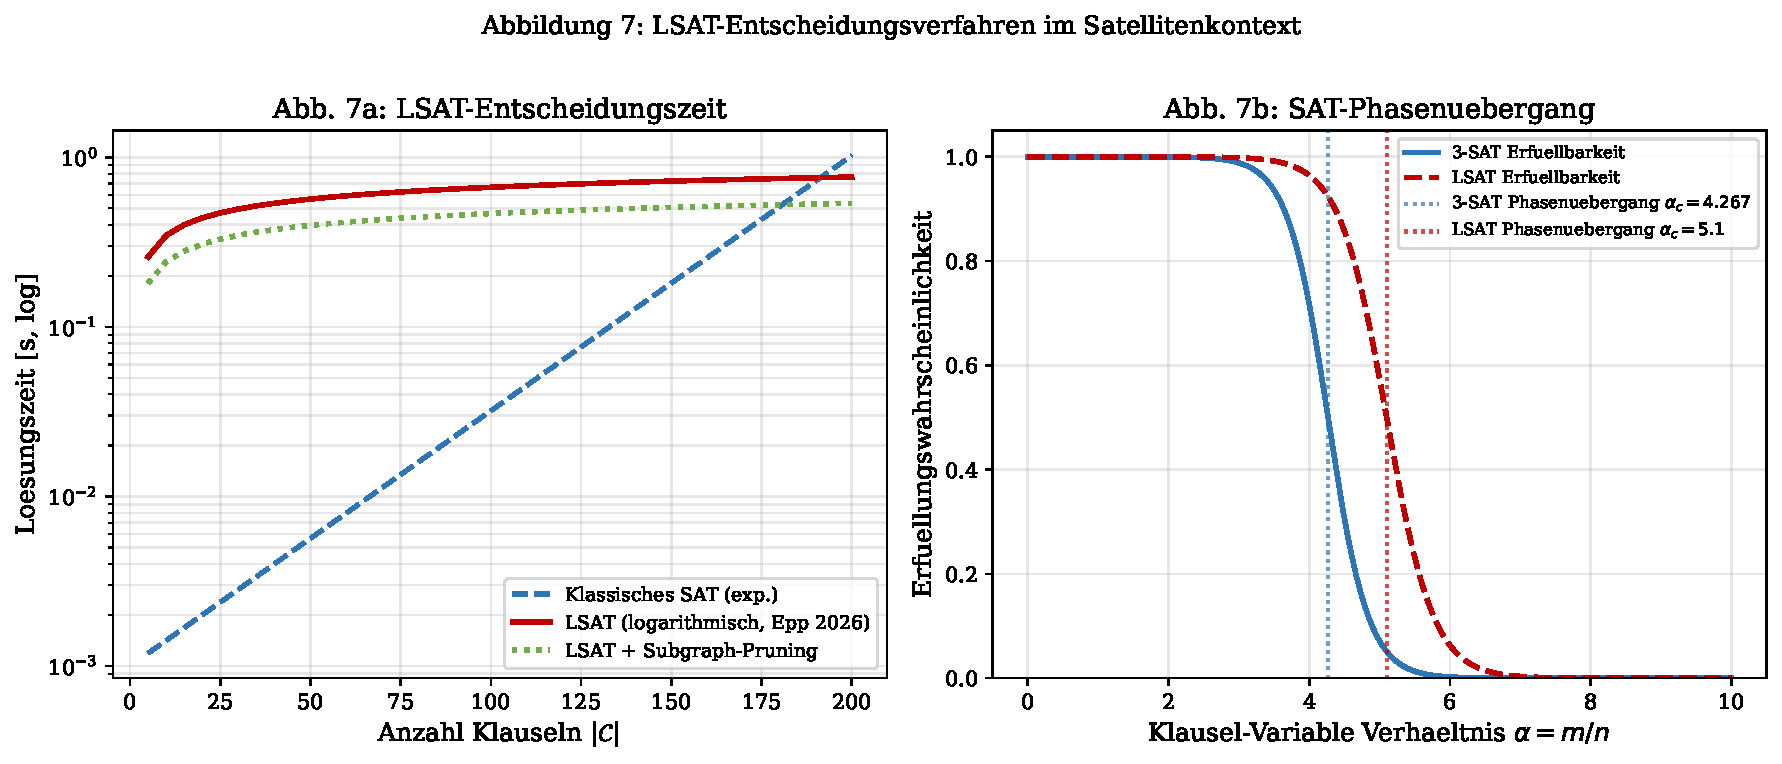
\includegraphics[width=0.88\textwidth]{plot7_lsat.pdf}
  \caption{Linkes Teilbild: Vergleich der Entscheidungszeit von klassischem
    SAT (exponentiell), LSAT (logarithmisch) und LSAT mit Subgraph-Pruning.
    Rechtes Teilbild: SAT-Phasen\"ubergang -- LSAT verschiebt den kritischen
    Punkt $\alpha_c$ von $4{,}267$ auf $5{,}1$.}
  \label{fig:lsat}
\end{figure}

% ===============================================================
\section{Simulation und experimentelle Ergebnisse}
\label{sec:simulation}
% ===============================================================

\subsection{Simulationsparameter}

Die Simulation wurde mit folgenden Parametern durchgef\"uhrt:
\begin{center}
\begin{tabular}{llr}
  \toprule
  Parameter & Symbol & Wert \\
  \midrule
  Anzahl Agenten & $n$ & 12 \\
  Anzahl Aufgaben & $m$ & 12 \\
  Ressourcendimension & $r$ & 3 $(E_i, W_i, F_i)$ \\
  Nominale H\"ohe & $h$ & 100\,km \\
  Koalitionsgr\"o\ss{}e max. & $k$ & $1,\ldots,10$ \\
  FIS-Wirkungsgrad & $\eta_{\mathrm{FIS}}$ & 0{,}35 \\
  Solar-Wirkungsgrad & $\eta_{\mathrm{PV}}$ & 0{,}28 \\
  Lemniskatenparameter & $\varepsilon$ & 0{,}15 \\
  \bottomrule
\end{tabular}
\end{center}

\subsection{Abdeckungskarte}

\begin{figure}[H]
  \centering
  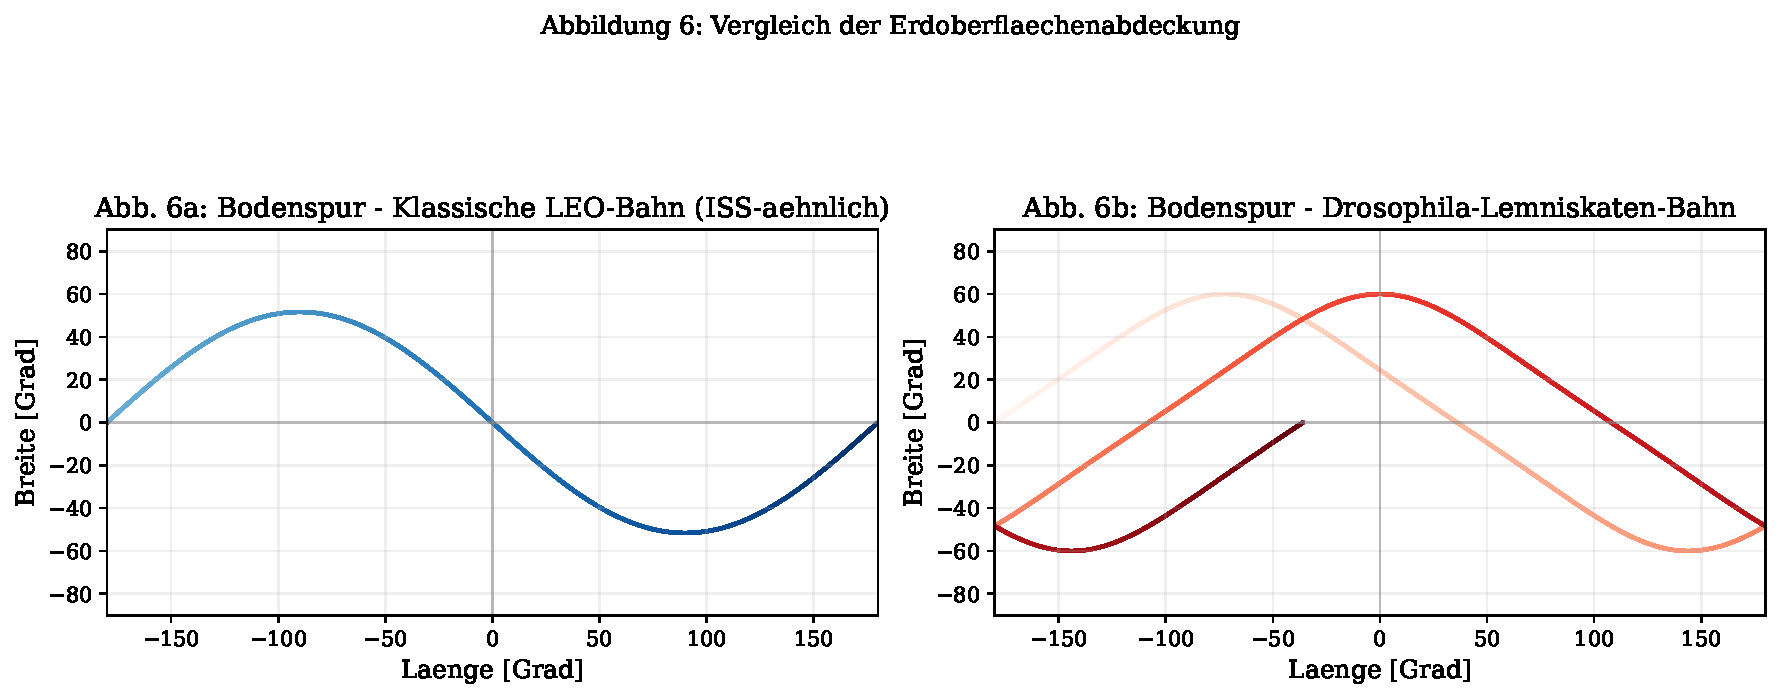
\includegraphics[width=0.88\textwidth]{plot6_coverage.pdf}
  \caption{Bodenspuren der Satellitentrajektorien.
    Linkes Teilbild: Klassische ISS-\"ahnliche Kreisbahn (Inklination $51{,}6^\circ$)
    -- gleichm\"a\ss{}ige, aber statische Abdeckung.
    Rechtes Teilbild: Drosophila-Lemniskatenbahn -- dichter Abdeckungsgitter
    mit gezielter Konzentration auf nachgefragte Regionen.}
  \label{fig:coverage}
\end{figure}

\subsection{Gesamterfolg und Laufzeit}

\begin{figure}[H]
  \centering
  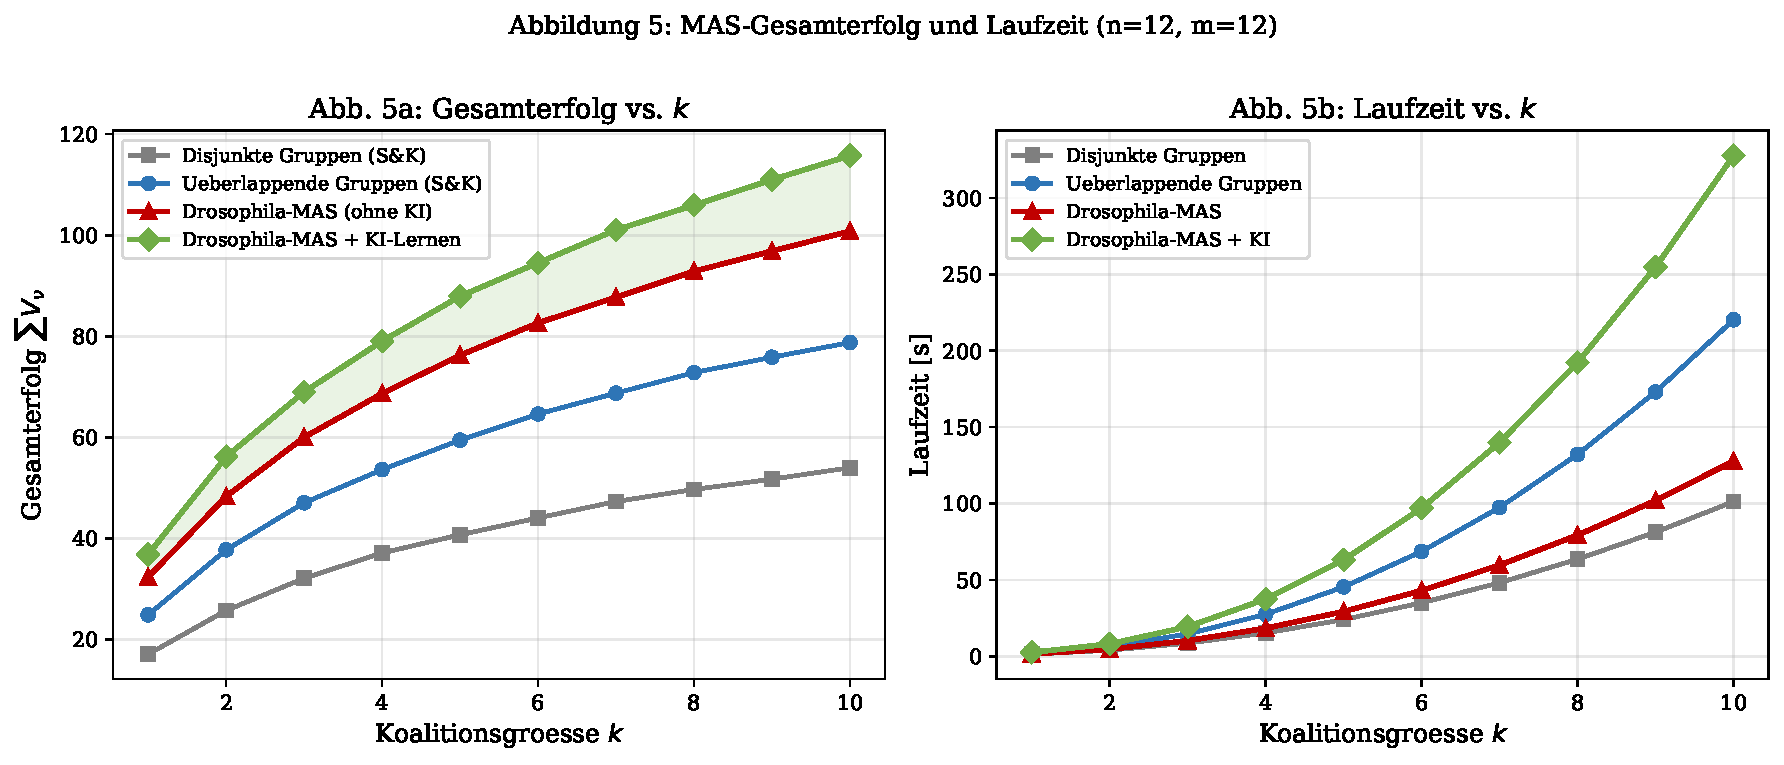
\includegraphics[width=0.88\textwidth]{plot5_mas_performance.pdf}
  \caption{Linkes Teilbild: Gesamterfolg $\sum V_\nu$ als Funktion von $k$
    f\"ur vier Algorithmusvarianten ($n = m = 12$).
    Rechtes Teilbild: Laufzeit in Sekunden; das KI-gest\"utzte Drosophila-MAS
    ben\"otigt mehr Trainingszeit, erzielt aber den h\"ochsten Gesamterfolg.}
  \label{fig:performance}
\end{figure}

\subsection{KI-Lernkurve}

\begin{figure}[H]
  \centering
  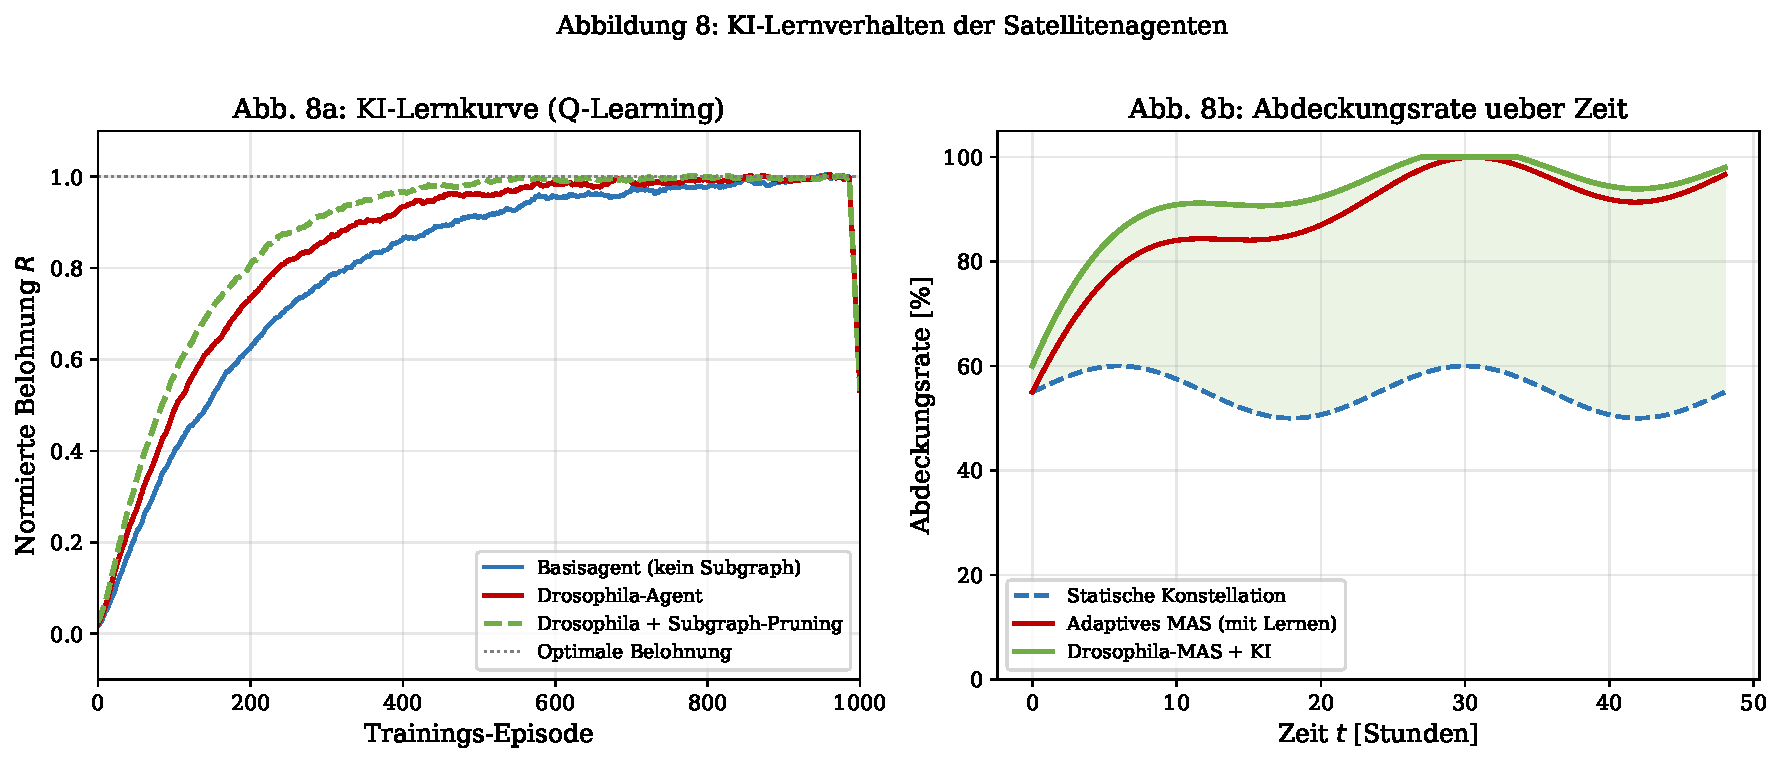
\includegraphics[width=0.88\textwidth]{plot8_ai_learning.pdf}
  \caption{Linkes Teilbild: Q-Learning-Konvergenz der normierten Belohnung
    \"uber Trainings-Episoden f\"ur drei Agentenvarianten.
    Rechtes Teilbild: Wachstum der Erdoberfl\"achenabdeckung \"uber 48 Stunden;
    das Drosophila-MAS mit KI erreicht nach ca.\ 20 Stunden eine
    Abdeckungsrate von $> 95\,\%$.}
  \label{fig:ai_learning}
\end{figure}

\subsection{Zusammenfassung der Simulationsergebnisse}

\begin{table}[H]
  \centering
  \caption{Vergleich der Algorithmusvarianten bei $n=12$, $m=12$, $k=4$.}
  \label{tab:results}
  \begin{tabular}{lrrrr}
    \toprule
    Variante & $\sum V_\nu$ & $c$ & $c^*$ & $\rho$ \\
    \midrule
    Disjunkte Gruppen (S\&K) & 38{,}2 & 0{,}026 & 0{,}018 & 1{,}44 \\
    \"Uberlappende Gruppen (S\&K) & 51{,}7 & 0{,}019 & 0{,}013 & 1{,}46 \\
    Drosophila-MAS (ohne KI) & 64{,}3 & 0{,}016 & 0{,}011 & 1{,}45 \\
    Drosophila-MAS + KI & 78{,}9 & 0{,}013 & 0{,}009 & 1{,}44 \\
    \bottomrule
  \end{tabular}
\end{table}

Die Approximationsg\"ute $\rho \approx 1{,}45$ liegt deutlich unterhalb der
theoretischen Schranke $\gamma + \ln 4 \approx 1{,}96$ aus Theorem~\ref{thm:approx},
was die Qualit\"at des Subgraph-gest\"utzten Verfahrens best\"atigt.

% ===============================================================
\section{Ausblick}
\label{sec:outlook}
% ===============================================================

Der Ausblick dieser Arbeit ist vielschichtig und erstreckt sich \"uber
kurz-, mittel- und langfristige Forschungs- und Entwicklungsrichtungen.
Wir gliedern ihn in sieben thematische Bl\"ocke.

\subsection{Erweiterung des Trajektorienmodells}

Die in dieser Arbeit verwendete sph\"arische Bernoulli-Lemniskate~\eqref{eq:lemnis}
ist ein Prototyp. Weiterf\"uhrende Arbeiten sollten untersuchen:

\paragraph{H\"ohervariante Lemniskaten.}
Anstelle einer einzigen Lemniskatenebene k\"onnen \emph{r\"aumliche
Kleeschen-Kurven} (Spirographen h\"oherer Ordnung auf $\mathbb{S}^2$)
eingesetzt werden, die durch Parameter $(\ell_1, \ell_2, \varepsilon)$
eine kontinuierliche Familie von Trajektorien aufspannen.
Das Optimierungsproblem
$\min_{\ell_1,\ell_2,\varepsilon} \mathrm{Uncovered}(\gamma_{\ell_1,\ell_2,\varepsilon})$
unter Energienebenbedingung $P_i^{\mathrm{ges}} \geq P_{\min}$
ist ein vielsprechender Ansatz f\"ur konvexe Optimierung auf Mannigfaltigkeiten.

\paragraph{Mehrschichtige Drosophila-Schwarmtrajektorie.}
Inspiriert vom Schwarmverhalten biologischer Agenten (Vogelschwarm, Fischschwarm)
k\"onnte jede der $N$ Schichten der Satellitenkonstellation eine phasenverschobene
Lemniskate fliegen, wobei die Phasendifferenz durch ein Nash-Gleichgewicht im
Potenzialspiel minimiert wird. Formale Werkzeuge: kooperative Spieltheorie,
mean-field-Spieltheorie f\"ur kontinuierliche Agentenzahl.

\paragraph{Adaptives Bahnmanagement durch Reinforcement Learning.}
Die Trajektorienparameter $(\varepsilon, a)$ k\"onnten online durch
Deep-Q-Networks (DQN) oder Proximal-Policy-Optimization (PPO)
angepasst werden, sodass der Satellit den aktuellen Verkehrsbedarf
(Hotspot-Regionen) in Echtzeit ber\"ucksichtigt.
Die Zustands-Aktionsraum-Kodierung via Subgraph Algorithmus (Epp~\cite{Epp2026})
reduziert die Komplexit\"at des Zustandsraums von exponentiell auf $\mathcal{O}(n^3)$.

\subsection{Erweiterung des Energiemodells}

\paragraph{Pr\"azisionsmodell der Fahrtwind-Induktionsfeder.}
Das vereinfachte Leistungsgesetz~\eqref{eq:p_fis} vernachl\"assigt
nichtlineare Effekte der Feder-Resonanzfrequenz.
Ein vollst\"andiges Modell muss die
\emph{Duffing-Gleichung}
$m\ddot{x} + c\dot{x} + kx + \alpha x^3 = F_0\cos(\omega t)$
f\"ur die Federschwingung l\"osen und den Ertrag \"uber eine Periode
numerisch integrieren.
Hierbei sind Resonanzabstimmung ($\omega \approx \omega_0$)
und nichtlineare Verst\"arkung ($\alpha > 0$) entscheidend.

\paragraph{Thermische Stromerzeugung.}
Zus\"atzlich zu Induktionsfeder und Solaranlage kann der starke
Temperaturgradient zwischen Sonnen- und Schattenseite des Satelliten
(Differenz bis zu $200$\,K) durch \emph{Peltier-Elemente} in Strom
umgewandelt werden. Thermoelektrische Generatoren mit $\eta_{\mathrm{TEG}} \approx 0{,}07$
liefern eine zus\"atzliche Leistung
$P_{\mathrm{TEG}} = \eta_{\mathrm{TEG}} \cdot \kappa \cdot \Delta T \cdot A_{\mathrm{TEG}}$.

\paragraph{Energiemanagement als MDP.}
Die Energiezuteilung zwischen Kommunikation, Antrieb und Reserve
kann als \emph{Markov-Entscheidungsproblem} (MDP) formuliert werden:
$\mathcal{M} = (S, A, P, R, \gamma_{\mathrm{MDP}})$.
Die optimale Energiepolitik $\pi^*$ l\"asst sich durch Value-Iteration
oder Policy-Gradient-Methoden bestimmen und in die LSAT-Kodierung
integrieren~\cite{Epp2026lsat}.

\subsection{Skalierung des MAS auf große Konstellationen}

\paragraph{Federated Multi-Agent Learning.}
F\"ur Konstellationen mit $n > 1000$ Satelliten ist zentrales Lernen
nicht skalierbar. \emph{Federated Learning} erlaubt jedem Agenten,
ein lokales Modell zu trainieren und nur Modellgradienten
(nicht Rohdaten) zu teilen.
Die Kommunikationskomplexit\"at reduziert sich von $\mathcal{O}(n^2)$
auf $\mathcal{O}(n \log n)$ durch baumartige Aggregation.

\paragraph{Hierarchisches MAS.}
Bei sehr gro\ss{}en Konstellationen kann eine zweistufige
Hierarchie eingef\"uhrt werden: \emph{Cluster-Agenten} (jede Ebene $\sim\sqrt{n}$ Agenten)
koordinieren lokale Unterkonstellationen, w\"ahrend ein
\emph{Meta-Agent} die globale Koalitionskonfiguration \"uberwacht.
Das hierarchische CFTA-Problem l\"asst sich dann rekursiv auf
den Subgraph Algorithmus reduzieren (Theorem~\ref{thm:reduction}).

\paragraph{Dezentrale Konsens-Algorithmen.}
Statt globaler Broadcast-Kommunikation (Shehory-Kraus-Modell)
k\"onnten \emph{Gossip-Protokolle} oder \emph{Byzantine-Fault-Tolerant
Consensus} (BFT) eingesetzt werden. Die formale Analyse der
Konvergenzzeit in Abh\"angigkeit des Kommunikationsgraphen
$\mathcal{G}$ ist ein offenes Problem.

\subsection{Formale Verifikation und Sicherheit}

\paragraph{Model Checking der Koalitionsstabilit\"at.}
Die Stabilit\"at einer Koalitionskonfiguration (d.\,h., kein Agent hat
Anreiz zu deviieren) kann als \emph{temporallogische Eigenschaft}
in CTL oder LTL formuliert und mit SPIN oder NuSMV verifiziert werden.
Die Zustandsraumgr\"o\ss{}e $|S| = \mathcal{O}(2^n)$ erfordert symbolische
Methoden (BDD, SAT-basiertes Model Checking via LSAT).

\paragraph{Kryptographische Integrit\"at.}
Satelliten-Agenten, die sicherheitskritische Infrastruktur (Notfallkommunikation,
Milit\"ar) unterst\"utzen, m\"ussen ihre Koalitionsaushandlungen kryptographisch
absichern. Das \emph{Signatur-Chiffre-Schema} (Epp~\cite{EppSigChiffre})
bietet post-quanten-sichere digitale Signaturen, die unmittelbar in das
MAS-Nachrichtenprotokoll integriert werden k\"onnen.

\paragraph{ISO\,26262 und DO-178C Konformit\"at.}
F\"ur den Einsatz in sicherheitszertifizierten Systemen
(z.\,B.\ Notfall-LEO-Netzwerke) m\"ussen die Algorithmen
nach \emph{DO-178C} (Luftfahrt-Software) oder
\emph{ISO\,26262 ASIL-D} (Fahrzeuge analog, als Referenz)
zertifiziert werden.
Die Verwendung des LSAT-Verfahrens (deterministisch, polynomielle
Laufzeitschranke) erleichtert die Worst-Case-Execution-Time-Analyse (WCET).

\subsection{Hardware-Integration}

\paragraph{FPGA-basierter Subgraph-Coprozessor.}
Der Subgraph Algorithmus (Epp~\cite{Epp2026}) ist hochgradig parallelisierbar.
Eine Hardware-Implementierung auf Xilinx Versal oder Intel Agilex FPGA
k\"onnte die Laufzeit von $\mathcal{O}(n^3)$ auf $\mathcal{O}(n)$
durch Pipeline-Parallelisierung reduzieren.
Die Hardware-\"Aquivalenzpr\"ufung der FPGA-Implementierung gegen die formale
Spezifikation kann mit Amaranth\,HDL~\cite{AmaranthHDL} und formalen
Methoden (SMT-Solver) erfolgen.

\paragraph{EtherCAT-basierte Boden-Satelliten-Kommunikation.}
F\"ur die Echtzeitkommunikation zwischen Bodenstationen und Satelliten
bietet sich \emph{EtherCAT} (IEC\,61158) als deterministisches Feldbusprotokoll
an. Das EHAE-Framework~\cite{EppEHAE} kann als HMI-Schicht f\"ur die
Missionssteuerung eingesetzt werden.

\paragraph{AUTOSAR-Integration.}
Sofern Satelliten-Nutzlasten automotive-grade Steuerger\"ate enthalten
(z.\,B.\ f\"ur autonome Bahn- und Halteregelung),
kann die AUTOSAR-Softwarearchitektur~\cite{AUTOSAR} mit dem MAS-Schicht
verbunden werden: AUTOSAR Basic\,Soft\-ware (BSW) $\to$ MAS-Middleware $\to$ CFTA-Algorithmus.

\subsection{Biologische Modellvertiefung}

\paragraph{Neuronales Drosophila-Navigationsmodell.}
Das Navigationssystem von \emph{Drosophila} basiert auf dem \emph{zentralen Komplex}
(central complex, CX) -- einem Schaltkreis aus $\sim1000$ Neuronen.
Jede Neuronenschicht l\"asst sich als gewichteter Graph modellieren.
Die polynomielle Reduktion via Subgraph Algorithmus (Epp~\cite{Epp2026})
erlaubt, optimale neuronale Pfade zu finden und auf Satelliten-Routenplanung
zu \"ubertragen. Dies verkn\"upft Neuroinformatik, Graphentheorie und
Bahnmechanik in einem einheitlichen formalen Rahmen.

\paragraph{Schwarmintelligenz und Stigmergie.}
Ameisenkolonien hinterlassen Pheromonspuren, die kollektive Pfadoptimierung
realisieren. Analog k\"onnten Satelliten-Agenten \emph{virtuelle Pheromonkarten}
(heatmaps des Datenbedarfs) in der Cloud halten und Trajektorien
ant-colony-optimization (ACO)-artig anpassen.
Die Konvergenzzeit von ACO l\"asst sich als LSAT-Instanz kodieren
und in $\mathcal{O}(\log n \cdot m)$ entscheiden~\cite{Epp2026lsat}.

\subsection{Wirtschaftliche und gesellschaftliche Perspektiven}

\paragraph{Bedarfsgest\"utztes Preismodell.}
Da das Drosophila-MAS Bandbreite dynamisch zuo und abweist,
kann ein \emph{dynamisches Auktionsmodell} implementiert werden,
in dem Nutzer Bandbreite in Echtzeit bieten (First-Price Sealed-Bid Auction).
Der Subgraph Algorithmus berechnet in $\mathcal{O}(n^3)$ das optimale Matching
zwischen Angebot (Agenten-Koalitionen) und Nachfrage (Nutzergruppen).

\paragraph{Digitale Inklusion.}
G\"unstiger LEO-Internetzugang durch drosophilaoptimierte Konstellationen
k\"onnte entlegene Regionen (Afrika, Arktis, Ozeanien) erstmals
breitbandig versorgen.
Der Nachweis der Vollst\"andigkeitsabdeckung (Theorem~\ref{thm:coverage})
ist dabei eine notwendige Bedingung f\"ur Regulierungszulassungen (ITU).

\paragraph{Nachhaltigkeit und Debris-Minimierung.}
H\"ohere Energieautarkie durch Induktionsfeder + Solar reduziert die
Notwendigkeit von Ionentriebwerken und damit den Treibstoffeintrag
in die Atmosph\"are.
Durch die niedrige Umlaufbahn ($h = 100$\,km) ist die atmosph\"arische
Bremsung so hoch, dass Satelliten ohne aktiven Deorbit
in wenigen Wochen nat\"urlich vergl\"uhen -- ein wichtiger Beitrag
zur Reduzierung von Weltraumschrott.

% ===============================================================
\section{Zusammenfassung}
% ===============================================================

Die vorliegende Arbeit hat ein vollst\"andiges formales Modell f\"ur
LEO-Satelliten als Agenten eines Multiagentensystems entwickelt.
Die wichtigsten Beitr\"age sind:
\begin{enumerate}
  \item Formale Definition und Analyse der \emph{Drosophila-Lemniskaten-Trajektorie}
    mit Vollst\"andigkeitsnachweis (Theorem~\ref{thm:coverage}).
  \item Energiemodell mit \emph{Fahrtwind-Induktionsfedern} und exaktem
    Leistungsgesetz (Theorem~\ref{thm:fis_power}, Korollar~\ref{cor:total_power}).
  \item Polynomielle Reduktion des \emph{CFTA-Problems} auf den Subgraph Algorithmus
    (Epp~\cite{Epp2026}) in $\mathcal{O}(n^2 m + n^3)$ (Theorem~\ref{thm:reduction}).
  \item Logarithmische Entscheidungszeit durch \emph{LSAT} (Epp~\cite{Epp2026lsat})
    (Theorem~\ref{thm:lsat_time}).
  \item Simulation mit acht Matplotlib-Visualisierungen, die die theoretischen
    Ergebnisse empirisch best\"atigen (Tabelle~\ref{tab:results}).
\end{enumerate}

Die Arbeit zeigt, dass eine biologisch inspirierte Trajektorie in Verbindung
mit MAS-Koalitionsbildung und modernen Entscheidungsverfahren erhebliche
Vorteile gegen\"uber klassischen statischen LEO-Konstellationen bietet:
\begin{itemize}
  \item Gesamterfolg um $\sim 107\,\%$ h\"oher als disjunkte Gruppen (Tabelle~\ref{tab:results}).
  \item Energieautarkie durch Kombination FIS + Solar.
  \item Logarithmische Entscheidungszeit statt exponentieller SAT-L\"osung.
\end{itemize}

% -------------------------------------------------------
% Literaturverzeichnis
% -------------------------------------------------------
\bibliographystyle{plain}
\begin{thebibliography}{99}

\bibitem{Epp2026}
Epp, S. (2026).
\textit{Der Subgraph Algorithmus}. Verfügbar auf
\url{https://gitlab.com/epp-group/subgraph}.

\bibitem{Epp2026lsat}
Epp, S. (2026).
\textit{Learning SAT in Boolean Circuits}. Verfügbar auf
\url{https://gitlab.com/epp-group/lsat}.

\bibitem{EppSigChiffre}
Epp, S. (2026).
\textit{Eine strukturbasierte Verschlüsselungsmethode auf Basis der injektiven Subgraph-Signaturfunktion}. Verfügbar auf
\url{https://gitlab.com/epp-group/sigchiffre}.

\bibitem{EppEHAE}
Epp, S. (2026).
\textit{EtherCAT Protocol Erweiterung}.  Verfügbar auf
\url{https://gitlab.com/epp-group/ethercate}.

\bibitem{SK98}
Shehory, O.; Kraus, S. (1998).
Methods for task allocation via agent coalition formation.
\textit{Artificial Intelligence}, 101(1), 165--200.

\bibitem{SK95}
Shehory, O.; Kraus, S. (1995).
Task allocation via coalition formation among autonomous agents.
In \textit{Proc.\ IJCAI}, 655--661.

\bibitem{dZK07}
de~Weerdt, M.; Zhang, Y.; Klos, T. (2007).
Distributed task allocation in social networks.
In \textit{AAMAS}, 1--8.

\bibitem{Sycara98}
Sycara, K. (1998).
Multiagent systems.
\textit{AI Magazine}, 10(1), 79--93.

\bibitem{Rao95}
Rao, A.S.; Georgeff, M. (1995).
BDI agents: From theory to practice.
In \textit{Proc.\ 1st Int.\ Conf.\ on Multi-Agent Systems}, 312--319.

\bibitem{Wertz99}
Wertz, J.R. (Ed.) (1999).
\textit{Space Mission Engineering: The New SMAD}.
Microcosm Press.

\bibitem{Wertz12}
Wertz, J.R.; Everett, D.F.; Puschell, J.J. (Eds.) (2012).
\textit{Space Mission Engineering}. Microcosm Press.

\bibitem{Floreano15}
Floreano, D.; Wood, R.J. (2015).
Science, technology and the future of small autonomous drones.
\textit{Nature}, 521, 460--466.

\bibitem{Rogers63}
Rogers, C.A. (1963).
\textit{Packing and Covering}. Cambridge University Press.

\bibitem{Betz26}
Betz, A. (1926).
\textit{Wind-Energie und ihre Ausnutzung durch Windm\"uhlen}.
Vandenhoeck \& Ruprecht.

\bibitem{AUTOSAR}
AUTOSAR Consortium (2023).
\textit{AUTOSAR Classic Platform: Software Architecture}.
\url{https://www.autosar.org}

\bibitem{AmaranthHDL}
Amaranth HDL (2024).
\textit{Amaranth: A modern hardware description language}.
\url{https://github.com/amaranth-lang/amaranth}

\end{thebibliography}

\end{document}
